\section{PCA - \textcolor{red}{P}rincipal \textcolor{red}{C}omponent \textcolor{red}{A}nalysis}
\begin{equation}
\mathbf{
    T = XP, \quad X = TP^T
}
\end{equation}
with residuals:
\begin{equation}
\mathbf{
T = XP + E, \quad \hat{X} = TP^T
}
\end{equation}

\textbf{P}: \quad Loadings \newline
\textbf{T}: \quad Scores \newline
\textbf{X}: \quad Original data \newline
\textbf{$\mathbf{\hat{X}}$}: \quad Projected data into reduced dimensions. \newline
\textbf{E}: \quad Residuals \newline

\textbf{PCA} is a linear transformation that finds the directions of maximum variance in the data. It projects the data into a new subspace.
\newline
\newline

\subsubsection{Deciding the number of components}
\subsubsection{Outlier detection}



\section{Some definitions from statistics}

\textbf{Covariance}: Covariance is a measure of the relationship between two
variables. A positive covariance means that the variables tend to increase
or decrease together, while a negative covariance means that the variables
tend to move in opposite directions. In other words, positive correlation
means ”if we measure an x that is bigger than its mean, then likely y will
be bigger too”\newline \newline
\textbf{Correlation}: The correlation coefficient, denoted by ”r”, is a value between
-1 and 1 that measures the strength and direction of the linear relationship
between two variables. A value of 1 means that there is a perfect positive
correlation (i.e. a perfect linear relationship) between the two variables, a
value of -1 means that there is a perfect negative correlation (i.e. a perfect
linear relationship with a negative slope) between the two variables, and a
value of 0 means that there is no correlation between the two variables.

\section{LS - \textcolor{blue}{L}east \textcolor{blue}{S}quares}
Least squares is about minimizing the sum of the squares of the differences between the observed and predicted values:
\begin{equation}
\min_{\theta} J(\theta) = \min_{\theta} \frac{1}{2m}\sum_{i=1}^{m} (\hat{y}_i(\theta)-y_i)^2
\label{eq:LS}
\end{equation}
A common way to predict the value of y is to use a linear model:
\begin{equation}
\hat{y} = \theta_0 + \theta_1x_1 + \theta_2x_2 + ... + \theta_nx_n
\label{eq:linear_model}
\end{equation}
\ref*{eq:LS} can solved numerically with \textbf{gradient descent}:
\begin{equation}
\theta_{j+1} = \theta_j - \alpha \nabla_{\theta} J(\theta)
\end{equation}
where $\alpha$ is the learning rate. \newline
In \textbf{Batch gradient descent} we use all the training examples in each iteration. In \textbf{Stochastic gradient descent} we use only one training example in each iteration.
\subsection*{Normal Equations}
If we assume a linear model like \ref{eq:linear_model} the least squares problem can be solved analytically with the normal equations. We fist have:
\begin{equation}
    \mathbf{
        y = X \theta}
\end{equation}
and
\begin{equation}
    \mathbf{
        X^T(\hat{y} - y) = 0 \quad
    }
\end{equation}
Substiting in $ \mathbf{\hat{y} = X \hat{\theta}} $ we get:
\begin{equation}
    \mathbf{
         \Rightarrow \quad X^T(X\theta - y) = 0 \quad \Rightarrow \quad X^TX\theta = X^Ty \newline
    }
\end{equation}
assuming the columns of X are linearly independent we get:
\begin{equation}
    \mathbf{
    \theta = (X^TX)^{-1}X^Ty
    }
    \label{eq:normal_equations}
\end{equation}

\section{Regularization}
Regularization is used to punish large values of the parameters $\theta$ in order to avoid overfitting. The most common regularization techniques are \textbf{L1} and \textbf{L2} regularization. When adding regularization you are trading off variance with some bias. (More about that in section xx) \newline

\subsection{L1 - LASSO}
L1 regularization adds the sum of the absolute values of the parameters to the cost function:
\begin{equation}
    \min_{\theta} J(\theta)_{new} = \min_{\theta} \quad J(\theta) + \lambda \sum_{j=1}^{n} |\theta_j|
\end{equation}


\subsection{L2 - Ridge}
L2 regularization adds the sum of the squares of the parameters to the cost function:
\begin{equation}
    \min_{\theta} J(\theta)_{new} = \min_{\theta} \quad J(\theta) + \lambda \sum_{j=1}^{n} \theta_j^2
\end{equation}

\subsection{Comparison between L1 and L2}
The L1 function look like a diamond and the L2 function look like a cone. The L1 function have higher chance of driving $\theta$ to zero, which is beneficial reducing model complexity. The L2 function will drive $\theta$ close to zero but not exactly zero. The L1 function is more computationally efficient to solve than the L function since J will in many cases remain convex.

\section{Preformance Metrics}
TODO

\section{Maximum Likelihood}
Maximum likelilihood is about fiting a distrebution to the observed data. It is about choosing both the parameters of the distrebution and the distrebution itself:
\begin {equation}
    \theta_{ML} = \arg \max_{\theta} P(X|\theta)
\end{equation}
The likelihood function is defined as:
\begin{equation}
    L(\theta) = P(X|\theta)
\end{equation}
The maximum likelihood estimator is the value of $\theta$ that maximizes the likelihood function. The log-likelihood function is often used since it is easier to work with:
\begin{equation}
    l(\theta) = \log(L(\theta))
\end{equation}

\section{Sampling}
Sampling is the process of selecting a subset of individual or items for a larger population for the purpose of analysis or study. We want to get a good represenation of the population with only a subset of the population. \newline
\subsubsection{Simple Random Sampling}
In simple random sampling, each individual is chosen entirely by chance and each member of the population has an equal chance of being included in the sample. It is impossible to sample truly randomly and it will cause low represenation of some subgroups. \newline

\subsubsection{Systematic Sampling}
In systematic sampling, the list of the population is ordered in some way and then the sample is chosen according to some pattern. This is done by selecting a random starting point and then picking every nth element in the list. Is not recomended if the population has a syclic pattern. \newline

\subsubsection{Cluster Sampling}
In cluster sampling, the population is divided into clusters and then a simple random sample of clusters is chosen. All individuals in the selected clusters are included in the sample. This is useful when the population is geographically spread out. \newline


\section{Bias-Variance Tradeoff}
\textbf{Ockham's razor} states that the simplest solution is often the best. The bias-variance tradeoff is about finding the right balance between bias and variance. \newline
Bias variance tradeoff can be calculated from the MSE:
\begin{equation}
    \mathbf{
    MSE = E[(\hat{\theta} - \theta)^2] = Bias^2 + Variance
    }
\end{equation}
Choosing model order is tightly connected to the bias-variance tradeoff. A model with high bias will underfit the data and a model with high variance will overfit the data. \newline
Regularization is reducing the variance by adding some bias. 



\section{DoE - \textcolor{green}{D}esign \textcolor{green}{o}f \textcolor{green}{E}xperiments}
Design of Experiments (DoE) is the pre-planned, systematic variation of
controllable experimental factors that induce a response in a system. The
factors are measured in such a way that the minimum effort is required to
gain a maximum amount of information.

The typical three stages of DoE are:
\begin{enumerate}
    \item \textbf{First screening}: The aim is to find main effect, \textbf{fractional factorial}.
    \item \textbf{Screening}: The aim is to find the main effects and interactions, \textbf{factorial}.
    \item \textbf{Optimization or oprtimal design }: Find optimal settings for a response surface, or design with constraints.
\end{enumerate}

\subsection{Experimental design vs OVAT - \textcolor{green}{O}ne \textcolor{green}{V}ariable \textcolor{green}{A}t a \textcolor{green}{T}ime}
In OVAT you change one variable at a time and keep the others constant. In this way you can not see the interactions between the variables. In experimental design you change all the variables at the same time. This is more efficient and you can see the interactions between the variables. \newline
\begin{figure}
    \centering
    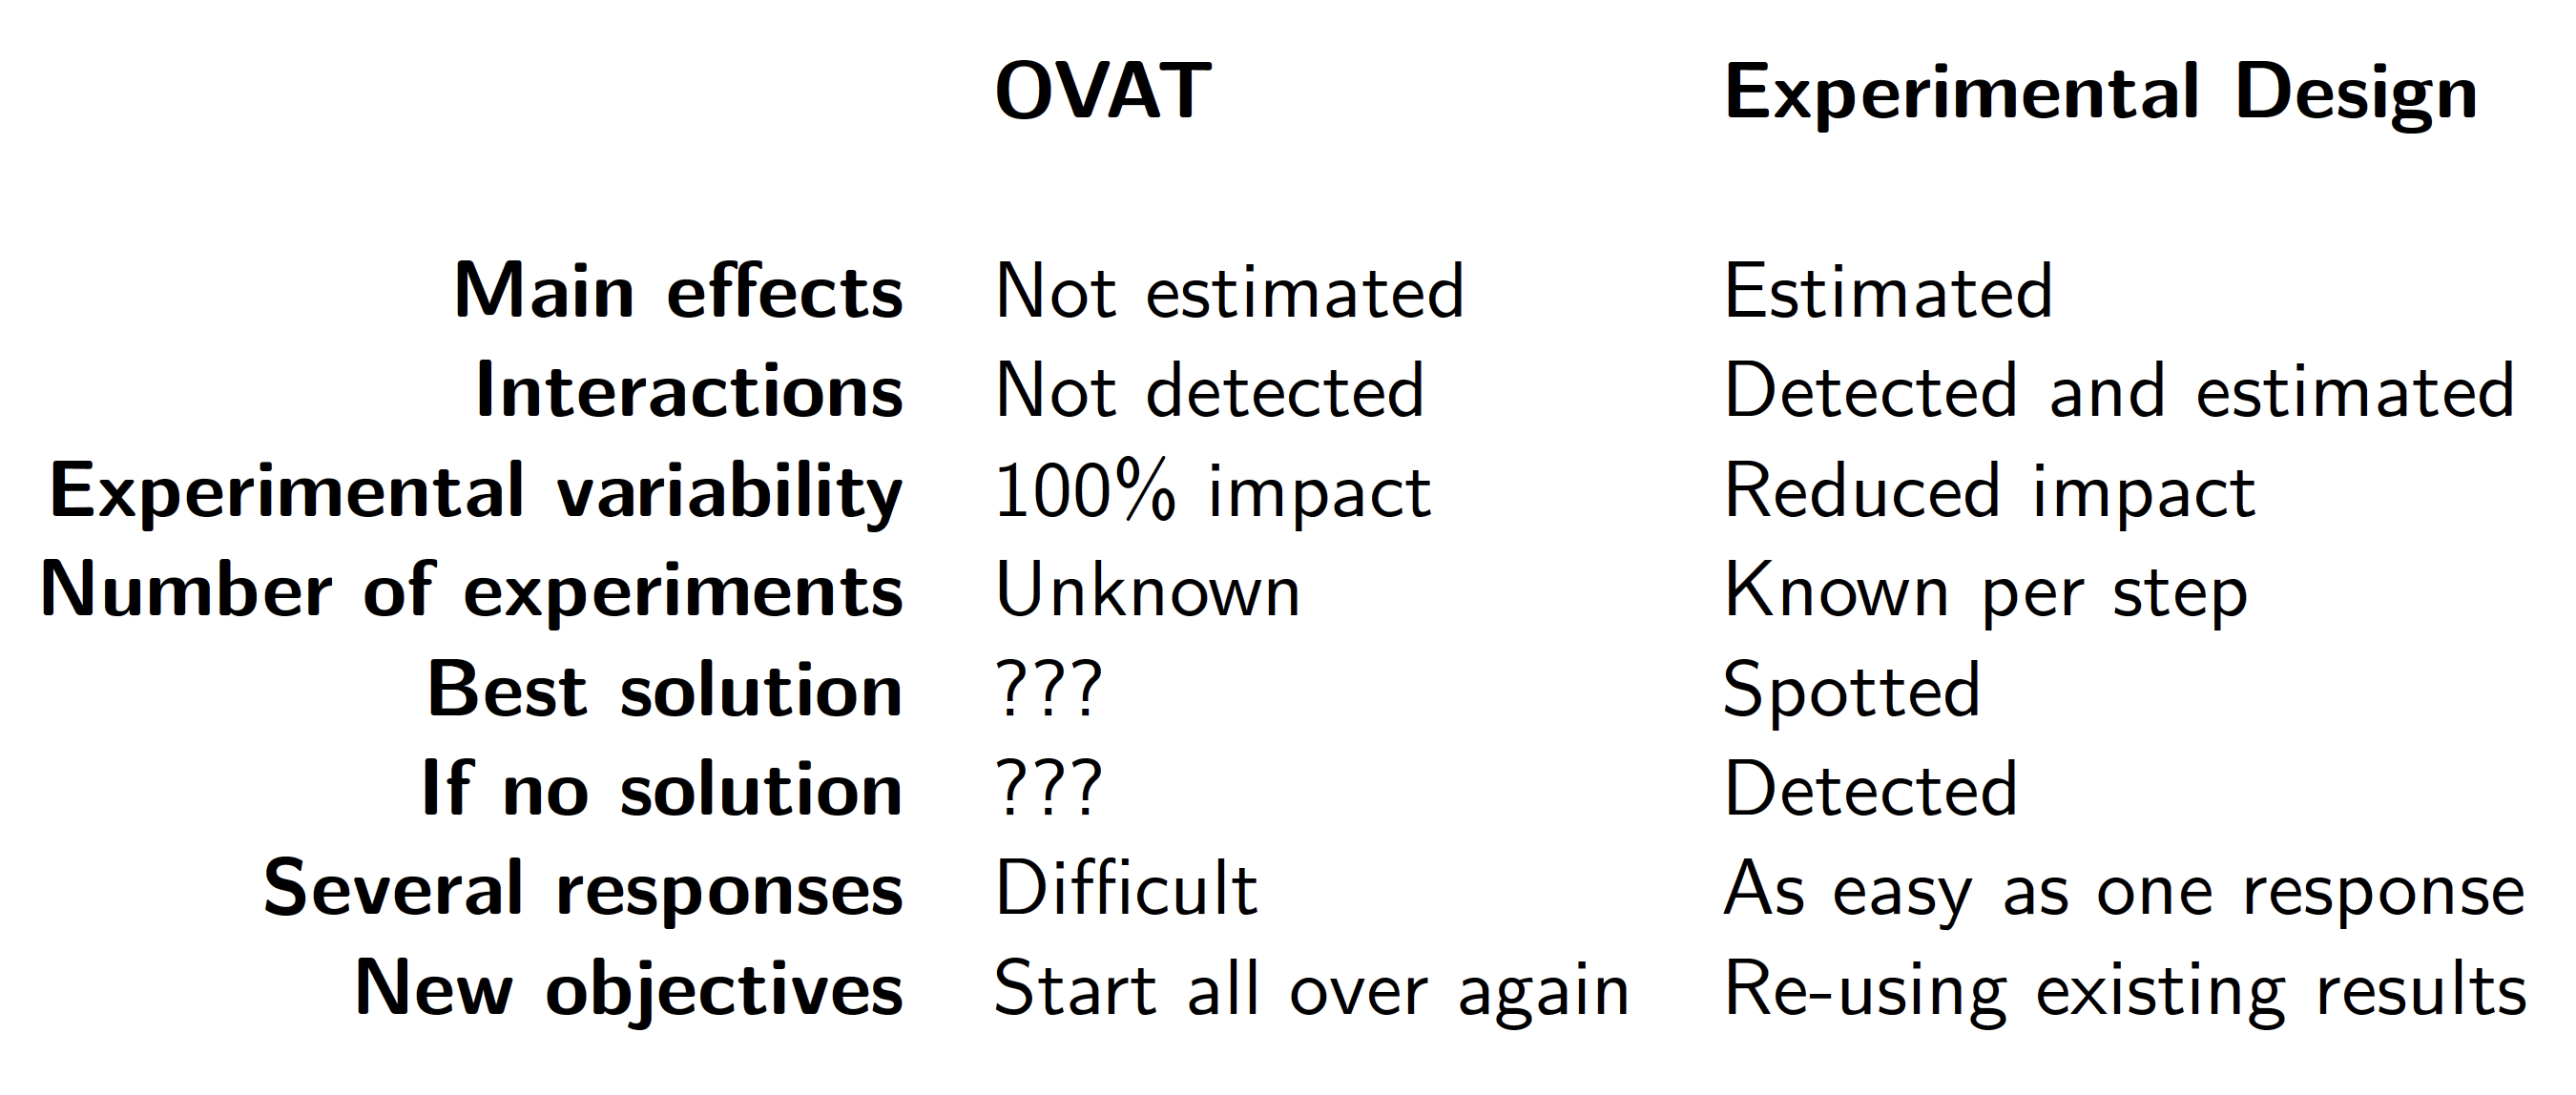
\includegraphics[width=1\textwidth]{pictures/OVAT_vs_ED.png}
    \caption{OVAT vs ED}
    \label{fig:OVAT_vs_ED}
\end{figure}

In full factorial, if you have two levels, high and low of each variable, the number of experiments needed is $2^n$ where n is the number of variables. \newline
In fractional factorial you only test $2^{n-1}$ experiments. \newline
Additionally it can be smart to add center samples to estimate curvature and estimate error variance. Antoher smart thing is to do replicated experiments to estimate the error variance. \newline

\section{ANOVA - \textcolor{green}{AN}alysis \textcolor{green}{O}f \textcolor{green}{VA}riance}

\section{MLR - \textcolor{blue}{M}ultiple \textcolor{blue}{L}inear \textcolor{blue}{R}egression}
MLR is used to model the relationship between a dependent variable and one or more independent variables. The model is defined as:
\begin{equation}
    \mathbf{
    y = \theta_0 + \theta_1x_1 + \theta_2x_2 + ... + \theta_nx_n
    }
\end{equation}
The parameters $\theta$ are estimated by minimizing the sum of the squares of the differences between the observed and predicted values. This is in practise the same as LS with a linear model; done by solving the normal equations \ref{eq:normal_equations}.
It is worth mentioning that if you have correlated X-variables the regression coefficient will not correspond to the true effect of the variable. (A negative $\theta_i$ does not mean that the variable has a negative effect on  y). You also have to have at least as many samples as variables in MLR. \newline


\section{PCR - \textcolor{red}{P}rincipal \textcolor{red}{C}omponent \textcolor{red}{R}egression}
The main idea of PCR is to use PCA to reduce the dimensionality of the data and then use MLR on the reduced data. The steps are:
\begin{enumerate}
    \item Do PCA on the X's.
    \item Choose the number of components to use.
    \item Do MLR on the reduced data.
\end{enumerate}
This is practical because the regression coefficients are interpretable aposed to normal MLR with potentioally correlated X-variables. It is also very practical since you can detect outliears in the predicition phase. However, in the PCA-phase the variance of X is only considered, nothing guarantees that the principal components which explained X
optimally could be relevant for the prediction of Y. \newline

\section{PLSR - \textcolor{red}{P}artial \textcolor{red}{L}east \textcolor{red}{S}quares \textcolor{red}{R}egression}
PLS tries to solve the problem of PCR by considering the covariance between X and Y. The model can be described as:
\begin{equation}
    \mathbf{
    X = TP^T + E
    }
\end{equation}
\begin{equation}
    \mathbf{
    Y = UQ^T + F
    }
\end{equation}
where:
\begin{itemize}
    \item loadings (\textbf{P}) and scores (\textbf{T}) in the \textbf{X} space.
    \item loadings (\textbf{Q}) and scores (\textbf{U}) in the Y space
    \item loading weights (\textbf{W}), eigenvectors maximizing the covariance between
    deflated Xa and Ya.
    \item errors (\textbf{E} and \textbf{F}) in the \textbf{X} and \textbf{Y} spaces.
\end{itemize}
\section{NlPALS - \textcolor{red}{N}on-\textcolor{red}{l}inear \textcolor{red}{P}artial \textcolor{red}{L}east \textcolor{red}{S}quares}

\section{Validation}

\subsection{External Validation}
External validation is validating that the model agrees with theory, that you can see causality.
\subsection{Internal Validation}
Internal validation is based on numerical methods like cross validation, test set validation and cross model validation. \newline


\section{Cross Validation}

\section{Outlier Detection}

\section{Feature Selection}

\section{SVM - \textcolor{blue}{S}upport \textcolor{blue}{V}ector \textcolor{blue}{M}achines}
SVM is an algorithm that can be used to both regression and classification. It is suited for non-linear problems and non-homogeneous classes. The main idea is to find the hyperplane that maximizes the margin between the classes. 
\indent \textbf{Hyperplane} is the decision boundary that is used to separate the data points of different classes in a feature space. In the case of linear classifications, it will be a linear equation i.e. wx+b = 0.
\newline \indent \textbf{Margin} is the distance between the support vector and hyperplane. The main objective of the support vector machine algorithm is to maximize the margin.  The wider margin indicates better classification performance.
\newline \indent \textbf{Support Vectors}: Support vectors are the closest data points to the hyperplane, which makes a critical role in deciding the hyperplane and margin.
\newline \indent \textbf{Kernel Trick}: In many cases it is impossible to separate the classes with a linear hyperplane. The data is therefor mapped into a higher dimension where it is more sepparable. The kernel trick is used to calculate the innerproducts without explicitly doing the mapping the samples into the higher dimension. A generic kernel function is defined as:
\begin{equation}
    K(x_a, x_b; \theta) = \text{function doing the implicit evaluation of the inner product}
\end{equation}
Where $\theta$ is a kernal hyper parameter.


\section{Timeseries Forecasting}

\subsection{Stationarity}
A process is said to be \textbf{strictly stationary} (or strongly stationary) if its statistical properties are invariant to shifts in time. This means that the joint probability distribution of the process does not change when shifted in time. \textbf{Wide sense stationary} is a less strict condition where the mean and variance is constant and the autocovariance function only depends on the time lag. Wide sence stationarity is a necessary condition for beeing able to predict the future.


\subsection{Ergodicity}
A process is said to be \textbf{ergodic} if the time average of one sequence is equal to the ensemble average of another sequence. This means that the statistical properties of the process can be estimated from a single, sufficiently long, realization of the process. \newline



\subsection {Decomposition of a timeseries}
A timeseries often consists of a trend, cyclic component, seasonale component and a residual. The trend is the long-term increase or decrease in the data. The cyclic component is the periodic fluctuations in the data. The seasonal component is the periodic fluctuations in the data that occurs at fixed intervals. The residual is the part of the data that is left after removing the trend, cyclic and seasonal components. Timese can be made out of addidative or multiplicative components. \newline


\subsubsection{FFT - \textcolor{blue}{F}ast \textcolor{blue}{F}ourier \textcolor{blue}{T}ransform}
FFT can be used to estimate the frequency content of a timeseries. It does assume that the timeseries is infinite and periodic and will therefore only give an approximation of the frequency content of the timeseries. A downside is that when the signal is converted to s-domain you no longer know at what time events are happening. A method to account for this is \textbf{windowed FFT} where you repeatadly do FFT over a sliding window. \newline

\subsubsection{Wavelet Transform}
Wavelet transform aim to solve the loss of time information in the FFT. The wavelet transform transforms a signal in time domain to a two-dimensional representation in time and frequency. In stead of decomposing the signal into sines and cosines of diffrent frequency, the wavelet transform decomposes the signal into wavelets of diffrent frequency \underbar{AND} diffrent time shift. Wavelets are in contrast to sines and cosines not periodic. 


\subsubsection{EMD - \textcolor{blue}{E}mpirical \textcolor{blue}{M}ode \textcolor{blue}{D}ecomposition}
EMD decomposes the timeseries into a finite number of \textbf{intrinsic mode functions} (IMFs). An IMF is a function that has satisfies:
\begin{enumerate}
    \item The number of extrema and the number of zero crossings must be equal or differ at most by one.
    \item At any point, the mean value of the envelope defined by the local maxima and the envelope defined by the local minima is zero.
\end{enumerate}
EMD can be described by:
\begin{equation}
    x(t) = \sum_{i=1}^{n} IMF_i + r
\end{equation}

Advantages of EMD:
\begin{itemize}
    \item works wit short time series.
    \item Can be used with non-stationary data.
    \item Can be applied to data representing non-linear processes.
    \item Works with non-periodic time series.
\end{itemize}
When preforming EMD you never leave the time domain. The IMFs are highly otrhogonal but not completely. The algorithm works as follows:
\begin{enumerate}
    \item Identify all the local maxima and minima of the signal.
    \item Interpolate between the maxima and minima to get the upper and lower envelope.
    \item Calculate the mean of the upper and lower envelope.
    \item Subtract the mean from the original signal.
    \item Repeat the process until the signal is a IMF.
\end{enumerate}

IMF - \textcolor{red}{I}ntrinsic \textcolor{red}{M}ode \textcolor{red}{F}unctions


\section{Multiway, multiblock and IDLE modelling}

\section{Clustering, classification and discrimination}

\section{DTW - \textcolor{blue}{D}ynamic \textcolor{blue}{T}ime \textcolor{blue}{W}arping}
Dynamic time warping is a similarity meassure between two time series. It is much used in speech and motion recognition. It is mathematically defined as:
\begin{equation}
DTW_q(x, x') = \min_{\pi \in \mathcal{A}(x, x')} \left( \sum_{(i,j) \in \pi} d(x_i, x'_j)^q \right)^{\frac{1}{q}}
\label{eq:DTW}
\end{equation}
\begin {itemize}
    \item $\pi$ is an \textbf{alignment path}, a series of K index pairs $(i_1, j_1), (i_2, j_2), ..., (i_K, j_K)$ where $i_k$ and $j_k$.
    \item $A(x, x')$ is the set of all possible $\pi$'s, satisying the following conditions:
    \begin{enumerate}
        \item The start and end is matched. $\pi_0 = (0,0)$ and $\pi_K = (n-1, m-1)$
        \item The index set is monotonic increasing and all datapoints must apear at least once.
    \end{enumerate}
    \item $q$ is the type of norm used to meassure the distance between the two time series.
    \item $d$ is the distance function.(probably).
\end{itemize}
$DTW(x,x) = 0$ and $DTW(x,x') > 0$ for $x \neq x'$. \newline
The optimization problem \ref*{eq:DTW} is solved by dynamic programming with complexity $O(nm)$ where $n$ and $m$ is the length of the two time series. \newline
It is worth mentioning that DTW is not a metric since it does not satisfy the triangle inequality. \newline

\begin{itemize}
    \item It can be used as a \textbf{pattern recognition tool} by predefining potential patterns and then compare the patterns to the time series. If the DTW is bellow a certain threshold the pattern is said to be present in the time series. \newline
    \item It can be used as a \textbf{feature extraction tool} by comparing the time series to a set of reference time series. Features can be distances to the reference time series, statistics from the alignment path etc.
    \item It can be used as a \textbf{anomaly detection tool} by comparing the time series to a set of reference anmaly series. If the DTW is bellow a certain threshold the time series is said to be an anomaly. 
\end{itemize}

\section{LDA - \textcolor{blue}{L}inear \textcolor{blue}{D}iscriminant \textcolor{blue}{A}nalysis}
LDA can be used to categorze between two or more classes. Assumtions are:
\begin{itemize}
    \item The classes are gaussian distributed.
    \item The classes have the same variance matrix $\Sigma$.
    \item The moments of the distributions can be estimated from the data.
\end{itemize}
Graphically LDA can be thought of as finding the line that maximizes the distance between the means of the classes and minimizes the variance within the classes. The line is called the \textbf{discriminant line} (discriminant loading(?)). The projection of the data onto the discriminant line is called the \textbf{discriminant score}. Afterwards a threshold $c$ can be set with to classify the data:

\begin{equation}
    discrimination test = \begin{cases} 
    \mathbf{w}^T \mathbf{x} \geq c \rightarrow class 1 \\ \\
    \newline
    otherwise class 2
    \end{cases}
\end{equation}

% \begin{equation}
%     X(\omega) = \begin{cases}
%     1 &\text{se $\omega\in A$}\\
%     1250 &\text{se $\omega \in A^c$}
%     \end{cases}
% \end{equation}


\section{QDA - \textcolor{blue}{Q}uadratic \textcolor{blue}{D}iscriminant \textcolor{blue}{A}nalysis}
If we remove the assumtion of $\Sigma_1 = \Sigma_2$ we get QDA. It is more complex to solve and LDA with quadratic feature engineering often give similar results.

\section{Model structure selection}

\section{PLS-DA - \textcolor{red}{P}artial \textcolor{red}{L}east \textcolor{red}{S}quares \textcolor{red}{D}iscriminant \textcolor{red}{A}nalysis}
If we have categorical y's PLS can be used as a classifications algorithm the following way:
\begin{enumerate}
    \item transform y's to $\hat{y}s$ by one hot encoding. (Perhabs use -1 and 1 instead of 0 and 1).
    \item do PLS on the $\hat{y}$'s and the X's.
    \item use new X's to predict with the model. Choose the class with the highest predicted value.
\end{enumerate}
The nice thing about this algorithm is that you get an associated probability with the prediction. \newline
Another nice thing is that you can study the correlation loadings to see which variables are most important for the diffrent classes. \newline

\section{PCA for classification}
PCA can be used as a classification algorithm for detecting cancer the following way:
\begin{enumerate}
    \item Do PCA on the X's (pixels) and generate score plot.
    \item Mark a area in the picture where the cancer is present and see where they correspond to in the score plot.
    \item Look at neighbouring pixels in the scoreplot and see if they are also cancerous.
\end{enumerate}

\section{t-SNE - \textcolor{blue}{T}-distributed \textcolor{blue}{S}tochastic \textcolor{blue}{N}eighbour \textcolor{blue}{E}mbedding}
A challenge with PCA isi that it captures the global struchture of the data. t-SNE aims to capture to local data and project it into a lower dimensional space.
\begin{itemize}
    \item \textbf{Neighbour Embedding}: The process of mapping high-dimensional data into a lower-dimensional space. The main idea here is to keep the distances between the data points in the lower dimenison as well. This is howerever generally not possible beacuse of whats called the \textbf{crowding problem}. Therefore only distances to "neighbouring" points are kept.
    \item 
\end{itemize}

\section{Clustering}
In a clustering promblem there are no predefined classes. The goal is to group similar data into clusters. Since we have no "solution" which we try to optimize to, it is an unsupervised algorithm. Clustering is wise to do prior to classification and also as EDA.

\textbf{Linkage Methods} are methods that uses a hierarchical approach to clustering. It is recursivly merging individual datapoints or exisisting clusters into new clusters based on a similarity meassure. The results of hierarcical methods can be visualized in a dendrogram. There clear bias variance tradeoff when choosing the number of clusters. It also important to be aware of "wishfull thinking" since you always can find a cluster if you look hard enough. The most common way to meassure similarity is through the euclidian distance. \newline

\subsubsection{K-means}
\begin{itemize}
    \item Simple and easy to implement
    \item Does not work with non-cicular clusters
    \item The number of clusters have to be predefined
    \item The algorithm is sensitive to the initial cluster centers, and must often be run multiple times with different initializations.
    \item You have to be aware of diffrent scaling on diffrent variables.
    \item "is bad" -Damiano.
\end{itemize}

\subsubsection{DBSCAN - \textcolor{blue}{D}ensity \textcolor{blue}{B}ased \textcolor{blue}{S}patial \textcolor{blue}{C}lustering of \textcolor{blue}{A}pplications with \textcolor{blue}{N}oise}
In DBSCAN you define a neighborhood $\epsilon$ which is a distance from a point. Diffrent types of points are defined as following:
\begin{itemize}
    \item \textbf{Core point}: A point that has many number of points within its $\epsilon$ neighborhood.
    \item \textbf{Border point}: A point that is within the that only has one neighbour.
    \item \textbf{Outlier}: A point that doesnt have any other neighbours.
\end{itemize}
The results of DBSCAN is not as dependent of $\epsilon$ as K-means is of the number of clusters. DBSCAN is also able to find non-circular clusters. \newline

\subsubsection{Visualizing clusters}
If you only have one cluster method and few samples you can use a \textbf{dendogram}. If you use two clusterers and have few samples you can use a \textbf{tanglegram}.


\section{ICA - \textcolor{red}{I}ndependent \textcolor{red}{C}omponent \textcolor{red}{A}nalysis}
The fact that the loadings in PCA are orthogonal can sometimes fail to describe the underlying structure of the data. In these cases ICA might be more appropriate. It is much used in signal processing to separate mixed signals. Let us say we have two audio signals $x_1$ and $x_2$ recorded at the same time. And that there are two sound sources $s_1$ and $s_2$ that are mixed together to form the signals $x_1$ and $x_2$. The mixing can be described as:
\begin{equation}
    \mathbf{
    x_1 = a_{11}s_1 + a_{12}s_2 
    }
\end{equation}
\begin{equation}
    \mathbf{
    x_2 = a_{21}s_1 + a_{22}s_2
    }
\end{equation}
This system of equations is underdetermined and we can not solve it directly. But if we assume:
\begin{enumerate}
    \item The sources are \textbf{independent}. $P(s_1,s_2) = P(s_1)P(s_2)$
    \item Maximum one of the sources are \textbf{non-gaussian}. This is because the central limit theorem states that the sum of independent random variables will be gaussian distributed. Its therefore impossible to separate the sources if they are both gaussian distributed.
    \item The A-matrix is \textbf{full rank}. This means that the sources are not mixed in the same way. You have to use different recordings.
\end{enumerate}
ICA can be applied. ICA can be interpreted through SVD:
\begin{equation}
    \mathbf{
    x = As  =  U\Sigma V^Ts \quad
    }
\end{equation}
$\mathbf{U}$ is a rotational matrix, $\mathbf{\Sigma}$ is a scaling matrix and $\mathbf{V^T}$ is a final rotational matrix. The angle of $\mathbf{U}$ is found by maximizing the variance. $\mathbf{\Sigma}$ is the covariance matrix and the angle of $\mathbf{V^T}$ is found by maximizing the Kurtosis. \newline \newline
It is wourth mentioning after preforming ICA the order of the components are arbitrary. You also get a scaling ambiguity. \newline


\section{Tree-based methods}
Tree-based methods require minimal preprocessing. They are computationally efficient and interpretable, but can easily overfit. The cost of predicting a sample with a trained model is the log of datapoints used to train. 
Decisiontrees can eaisly visualize feature importance of the model. Small variations in dataset will lead to compleatly different trees, and Skewed datasets can lead to biased trees. \newline
In practise they work by asking a series of questions that maximizes the information gain:
\begin{equation}
    Information \quad gain = Entropy_{parent} - \frac{1}{N}\sum_{i=1}^{n} Entropy_{child_i}
\end{equation}
where the entropy is defined as:
\begin{equation}
    Entropy = -\sum_{i=1}^{n} p_i \log_2(p_i)
\end{equation}
And can be thought of as a measure of purity. \textbf{Random forests} is an ensemble method that uses multiple decision trees to improve the accuracy of the model. \newline
The features are selected randomly and the trees are trained on different subsets of the data. The final prediction is the average of the predictions of the individual trees.


\section{Logistic regression}
Logistic regression is used when the target variable is binary. It is therefore a classification algorithm.
Logistic regression can be used for digit recognition. The algorithm is esentially a linear regression model with a sigmoid function applied to the output. The sigmoid function is defined as:
\begin{equation}
    \mathbf{
    \sigma(z) = \frac{1}{1+e^{-z}}
    }
\end{equation}

\section{Neural networks}
Neural networks are essentially a series of logistic regression models. Neural networks also has the ability to approximate any countinuous function. This is known as the \textbf{universal approximation theorem}. The most common activation functions are the sigmoid function, the hyperbolic tangent function and the rectified linear unit function. The sigmoid function is used in the output layer of a binary classification problem. The hyperbolic tangent function is used in the output layer of a multi-class classification problem. The rectified linear unit function is used in the hidden layers of the network. If you remove the activation function you are essentionally left with a linear model. \newline
The gradient is calculated by an algorithm called \textbf{backpropagation}. Neural network can handle non linear relationships between the input and output variables. It is woth mentioning that  they can be prone to overfitting and can be computationally expensive to train. It can also be difficult to find a global minimum. \newline
To avoid overfitting you can use \textbf{dropout} which is a technique where you randomly set a fraction of the neurons to zero. $L_1$ and $L_2$ regularization can also be used. \newline
\textbf{Early stopping} is a technique where you stop training the model when the validation error starts to increase. \newline
Because of chain rule an unwanted effect of the backpropagation algorithm is the \textbf{vanishing gradient problem}. This can be solved by using ReLU instead of the sigmoid function. \newline
Another drawback og neural networks is that they are often considered as black boxes, hard to interpret.

\subsection{CNN - \textcolor{blue}{C}onvolutional \textcolor{blue}{N}eural \textcolor{blue}{N}etworks}
CNN is a type of neural network that is most used in image recognition. The main idea is to use convolutional layers to extract features from the image. \textbf{max pooling} is used to reduce the dimensionality of the image. The output of the convolutional layers is then fed into a fully connected layer which can be used for classification. \newline

\subsection{Autoencoders}
Autoencoders are a type of neural network that is used for dimensionality reduction. The main idea is to train the network to output the input. The network is trained to minimize the difference between the input and the output. The network is trained to learn a compressed representation of the input. The compressed representation is called the \textbf{latent space}. The latent space can be used for clustering, classification and anomaly detection. \newline














